% Chapter 1

\chapter{Batteries --- an introduction} % Main chapter title
In this chapter, a brief description has been made on the parameters required for understanding a battery performance and various types of batteries available in current market.   
\label{chap1} % For referencing the chapter elsewhere, use \ref{Chapter1} 

%----------------------------------------------------------------------------------------

% Define some commands to keep the formatting separated from the content 
\newcommand{\keyword}[1]{\textbf{#1}}
\newcommand{\tabhead}[1]{\textbf{#1}}
\newcommand{\code}[1]{\texttt{#1}}
\newcommand{\file}[1]{\texttt{\bfseries#1}}
\newcommand{\option}[1]{\texttt{\itshape#1}}

%----------------------------------------------------------------------------------------
According to an IEA estimate, we humans produced and used 5.67 x 1020 joules of energy in 2013, equivalent to about 18.0 terawatt-hour (TWh). One TWh is equivalent to 5 billion barrels of oil per year or 1 billion tons of coal per year, it also used to be the globe's entire energy consumption in 1890.
A photovoltaic (PV) produces power only while sunlight is available. Grid provides electricity when the sun is shining, and at night or during periods of cloudy weather. However, storage should be included in grid-connected systems to increase the value of the PV-generated electricity. In the grid connect systems, batteries prove favorable when used for daily peak-demand reserve. 
Every energy storage device can be used for a specific purpose (a capacitor can be used for short-term storage). Batteries store energy in a chemical form. Its maintenance and parameters like battery lifetime , available power and efficiency, play a significant role while maintaining a grid-connected systems operation. Batteries have various advantages and can be used for multiple purposes. In grid-connected systems, a battery can be used to store the power generated by the sun for several hours in order to match when peak load occurs. Specific capacity and battery potential are one of the most important battery performance indicators. It is important that we understand these and a few other terms to completely understand a battery. 
\begin{itemize}
\item \textbf{Battery capacity}: Battery capacity is the amount of charge or energy stored in it. Mathematically, it is evaluated by integrating current over time. The fundamental units of battery capacity is coulombs (C), though Amp-hrs (Ah) is more commonly used.  Theoretical capacity (ideal capacity under equilibrium conditions) is calculated with the help of chemical reactions that take place inside the cell. The equation gives us number of moles of the active species and number of participating electrons, \textit{n}. Using Faraday’s constant (number of Coulombs per mole of electrons, F = 96,484.56 C mol$^{-1}$), total available charge can be calculated for a battery. The capacity when described in Ah can be determined using the equation:
\begin{equation} \label{eq1}
  \text{Capacity(Ah)}=\frac{n \times F \times 1 \text{ hour}}{3600 \text{ sec}}
\end{equation}
\item \textbf{Battery potential}: Voltage is the  most important characteristic of a battery. Various factors help determine a cell's voltage such as electrolyte stability, polarization of the battery and concentrations of the active species. Figure \ref{Figures/chap1fig:CDCforcellvoltage} represents an ideal charge/ discharge curve (CDC). To avoid any permanent damage, a battery should not be discharged below a certain level. This voltage is called the "cut-off voltage". Upper and lower cut-offs depend on the electrolyte stability. Going beyond these potentials might lead to certain reactions that decompose the electrolyte (also called side reactions) resulting in an irreversible capacity loss. 
\begin{figure}[tbh!]
\centering
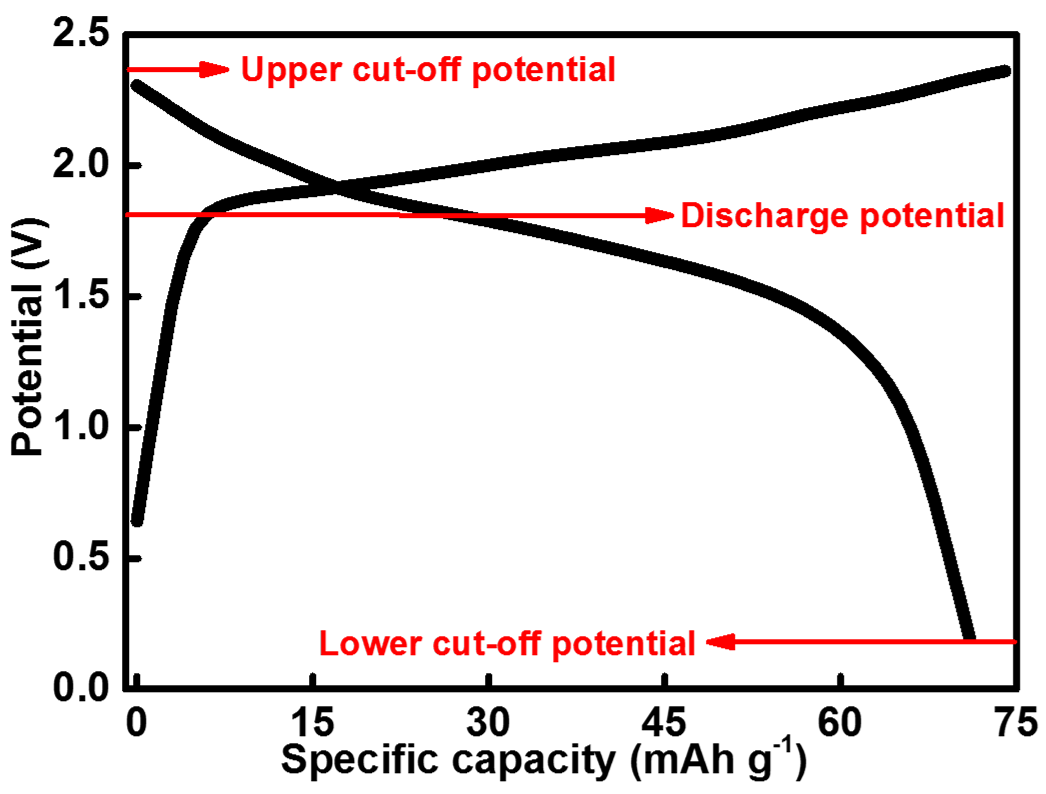
\includegraphics[width=\textwidth]{Figures/chap1fig/CDCforcellvoltage}
\caption{A charge/ discharge curve of an aluminium ion cell using graphite as the cathode and pure aluminium as the anode. The cell was charged and discharged to 2.45 V and 0.2 V respectively.}
\label{Figures/chap1fig:CDCforcellvoltage}
\end{figure}
    %While the reduction of battery voltage with discharge is a negative aspect of batteries which reduces their efficiency, one practical aspect of such a reduction, if it is approximately linear, is that at a given temperature, the battery may be used to approximate the state of charge of the battery. In systems where the battery voltage is not linear over some range of state of charge of the battery or in which there are rapid variations in the voltage with the BSOC will be more difficult to determine the BSOC and therefore will be more difficult to charge. However, a battery system that maintains a more constant voltage with discharge rate will have a high voltage efficiency and will be more easily used to drive voltage sensitive loads. Battery voltage will increase with the temperature of the system, and can be calculated by the Nernst Equation for the equilibrium battery voltage.
    
\item \textbf{Energy density}: The primary function of a battery is to store electrical energy. It is an important characteristic of a battery for any portable application, whether it’s for a laptop or an electric vehicle. Heavy batteries required to move something as large as a car over long distances need high energy density batteries. We need battery chemistries which have higher theoretical energy densities than Li-ion batteries, the current state-of-the-art. A simple way to determine the specific energy or energy density of a battery is using Eq.\ref{eq2} multiply the capacity by the battery voltage:
\begin{equation} \label{eq2}
    \text{Energy Capacity}= \text{Ah} \times \text{Battery voltage}
\end{equation}
\item \textbf{Power density}: Power density measures how quickly a battery can deliver energy. Also known as specific power, it's equivalent to the maximum current one can draw from a battery. Units used to describe power density are W kg$^{-1}$ or W m$^{-3}$. The best way to differentiate between energy and power density of a battery is to use an example of a moving car. Energy density determines how 'far' the car will go, whereas power density determines how 'fast' the car will go.
\item {\textbf{Primary and secondary batteries}}: Primary or non-rechargeable batteries produce current immediately when assembled. They have very high energy densities since it is a single-use system. Implanted medical devices, guided missiles, mars rovers and military ordnance use primary batteries. They have a low initial cost, however disposing a primary cell is problematic since the chemical reactions are not easily reversible and active materials may not return to their original states. They prove to be an uneconomical energy source since they produce only about 2\% of the power used during their production. Common types of disposable batteries include zinc–carbon and alkaline batteries. 
\textit{Secondary}, or rechargeable batteries, need to be charged before their first use. Applying an electric current (during charge) reverses the cell's active materials chemical state since they are  assembled in the discharged state. Since they can store energy reversibly, they are extensively used as energy storage devices. The oldest form of rechargeable battery is the lead–acid battery, which has been used since the 1700's. These batteries find extensive use in automotive, power tools, laptop computers, mobile phones, toys, etc. The most commonly used examples of rechargeable batteries are lithium-ion batteries, nickel-cadmium (NiCad) and nickel metal hydride (NiMH) batteries. 
\item \textbf{Coulombic efficiency}: Coulombic efficiency of a battery is the ratio of number of charges that enter during charge to the number that can be extracted from the battery during discharge.  Any loss in coulombic efficiency can be attributed to some secondary reaction (side reactions) in the battery system. A high coulombic efficiency in excess of 95\% is considered a standard value for commercial battery systems.
  
    \end{itemize}
The charging/discharging rates affect the rated battery capacity. If the battery is being discharged very quickly (i.e., the discharge current is high), then the amount of energy that can be extracted from the battery is reduced and the battery capacity is lower. This is due to the fact the necessary components for the reaction to occur do not necessarily have enough time to either move to their necessary positions. The only a fraction of the total reactants are converted to other forms, and therefore the energy available is reduced. Alternately, is the battery is discharged at a very slow rate using a low current, more energy can be extracted from the battery and the battery capacity is higher. Therefore, the battery of capacity should include the charging/discharging rate. A common way of specifying battery capacity is to provide the battery capacity as a function of the time in which it takes to fully discharge the battery (note that in practice the battery often cannot be fully discharged). The notation to specify battery capacity in this way is written as C$_x$, where x is the time in hours that it takes to discharge the battery. In the above table, C$_{10}$ (also written as C$_{10}$ = xxx) means that the battery capacity is xxx when the battery is discharged in 10 hours.The temperature of a battery will also affect the energy that can be extracted from it. At higher temperatures, the battery capacity is typically higher than at lower temperatures. However, intentionally elevating battery temperature is not an effective method to increase battery capacity as this also decreases battery lifetime. 
An ideal battery should be low-cost, get charged and discharged indefinitely under high or low current rate, have a long lifetime with high coulombic efficiency (>95\%), high energy density, and low-self discharge. However, it is very difficult to achieve the above set of requirements. Researchers are working towards various chemistries to achieve the above set of requirements. The lithium-ion battery system is a power pack of choice not only on the Earth, but also in space. It receives the most attention and is gradually replacing the nickel-based predecessors that dominated the battery world until the 1990s. Last year in October, a few astronauts on board the International Space Station (ISS) finally stepped outside their quarters for a spacewalk. Flight engineers Christina Koch and Jessica Meir (first all female spacewalk) were assigned the task of manually swapping out two nickel hydrogen (NiH) batteries for one brand new lithium-ion battery (LIB). This would not only upgrade the station's complex electrical system but also extend it's life through 2020's. ISS was launched into orbit in 1998 with 48 NiH batteries. The National Aeronautics and Space Administration (NASA) has started swapping these old batteries, since 2017, with 24 new LIBs  that provide higher energy density and a better power efficiency. Naturally, they had to be careful while handling these heavy batteries (195 kg) because they cannot be damaged or dented. LIBs come with a potential risk of \textit{thermal runaway}- defects or manhandling a battery to overheat and explode. Inside a pressurised oxygen-rich capsule, the results would have been catastrophic! NASA has found a solution for this safety concern by making batteries equipped with materials that would contain any form of leakage and prevent if from emitting heat , smoke or fire in case of combustion. 
A battery expert said that the switch from lead acid to Li-ion will be faster than the advancement of the Internet. Applied to a battery, Moore’s Law would shrink a starter battery in a car to the size of a coin.
\section{Rechargeable batteries and other power sources}
\subsection{Lead-acid batteries}
Lead acid batteries are the most commonly used type of battery in photovoltaic systems. Although lead acid batteries have a low energy density, only moderate efficiency and high maintenance requirements, they also have a long lifetime and low costs compared to other battery types. One of the singular advantages of lead acid batteries is that they are the most commonly used form of battery for most rechargeable battery applications (for example, in starting car engines), and therefore have a well-established established, mature technology base.
\subsection{Nickel-cadmium (NiCad)}
Nickel-cadmium may be cost effective on a life-cycle/cost basis. They consist of a positive electrode of nickel (or hydroxide) and a negative electrode of cadmium hydroxide. They are commonly used in a sealed configuration in small household appliances. NiCad batteries have several advantages such as a long lifetime and long storage life. The redox processes occur on the surface of the electrodes which means there is no loss of the active material. These processes increase the cell's lifetime. Furthermore, the electrolyte in nickel-cadmium is less corrosive to battery parts than in a lead-acid battery which also increases lifetime. A NiCad cell can be fully discharged and charged without damaging the battery. NiCad batteries are less sensitive to colder temperature, tolerating temperatures of -50$^{\circ}$C. In addition, the NiCad batteries have low maintenance requirements. Unlike, lead-acid batteries, NiCad batteries do not use corrosive elements and require less frequent maintenance. However, they also have a number of disadvantages. Some of the disadvantages include; Expense. Nickel-cadmium batteries are typically at least twice as expensive than lead-acid batteries and record lower coulombic efficiencies between 75\% to 85\%.

\subsection{Vanadium redox-flow batteries)}
 Redox flow batteries use a reduction-oxidation between two valence states in solution rather than changing the composition, and hence the valence states of solid material on an electrode. A flow battery consists of two volumes of solution separated by a selective membrane which allows some ions to pass but not others. Flow batteries have several potential advantages over solid batteries. A key advantage, which is particularly important in transport applications, is that the battery may be re-charged simply by pumping out the uncharged solution and replacing the solution with charged solution. This eliminates potentially long recharging times, such as are encountered in electric vehicles. Replacement of the solution allows the electric car to be recharged in the same fashion in which a car is filled with fuel. Another advantage is that the capacity of the battery is determined by the volume of solution, while the power of the battery is determined by the membrane contact area between the two solutions. The vanadium-Vanadium redox flow battery, developed at the University of New South Wales, is a particularly promising flow battery. It consists of two states of Vanadium. It has high efficiencies, with coulombic efficiencies of 97\% and energy efficiencies of 87\%. In addition, since both solutions (anode and cathode) in the battery use vanadium, cross contamination between the two solutions may discharge the battery, but will not cause damage to the battery.
\subsection{Lithium and lithium-ion (LIB)}
An electrochemical potential is a measure of the energy of the outer most electrons. Examination of the electronic configuration of the outer shell of the material gives an indication of the magnitude and sign of the electrochemical potential between the reactants and products of a redox reaction taking place inside a battery. The standard potential of a redox reaction is used to determine if a redox reaction will occur spontaneously (if it will generate a voltage between the reduction and oxidation reaction). If the difference between the standard potentials is positive, then the reaction will proceed spontaneously. If the standard potential is negative, a voltage needs to be applied in order for the reaction to proceed, which is precisely what is needed in a battery. Therefore, standard potential is an important parameter to find a suitable battery anode. Lithium has the highest electrochemical potential. It can achieve very high energy and power densities in high power battery applications. Many variations (such as lithium-ion) of the basic lithium chemistry have been developed for specific applications. Lithium is a highly flammable metal. Early commercial cells with metallic lithium cathodes were considered unsafe because of this property. However, modern cells use compounds of lithium that do not react as aggressively. A typical Li-ion cell use graphite for its anode and lithium-cobalt dioxide (LiCoO$_2$) or a lithium-manganese compound (\ce{LiMnO4}, \ce{Li2MnO3}) as cathodes. An electrolyte is a medium that allows ion-transfer inside the cell. The most commonly used electrolyte for LIBs is based on \ce{LiPF6} and mixtures of cyclic and linear carbonate solvents. The linear carbonates, such as dimethyl carbonate (DMC), ethyl methyl carbonate (EMC), or diethyl carbonate (DEC), maintain low viscosity of the electrolyte and enhance its conductivity. However, they are flammable and show flash points around room temperature (between 16 and 33$^{\circ}$C). In combination with an oxidant and an ignition source, they may catch fire and cause explosions. Using non-flammable electrolyte solvents or of flame-retardant electrolyte additives enhances the safety of flammable electrolytes, it deteriorates the electrochemical performance of batteries. 
However, LIBs have become the leading pioneers in battery technology especially for portable consumer electronics. Additionally, volume production has brought the prices down.
Mechanisms: 1. Intercalation/ deintercalation, 2. alloying/ dealloying 
\section{Aluminium-ion battery}
To find a suitable battery system, one needs to examine theoretical specific capacities of different ions that can replace lithium, using \ref{eq1}. Metals in the upper left corner of the periodic table, such as sodium (Na), magnesium (Mg), potassium (K) and calcium (Ca) reported higher theoretical capacities than the others and can be alternatively used as battery anodes. Table  \ref{table1} shows calculations for a few common metal anodes. 
\begin{table}[tbh!]
\caption{Comparing important parameters of various metal anodes.} \label{table1}
\begin{tabular}{lccccrr}
\headrow
\hline
 & \textbf{Li} & \textbf{Na} & \textbf{Mg} & \textbf{Al} & \textbf{K} & \textbf{Ca}\\
\hline
Valence electrons & 1 & 1 & 2 & 3 & 1 & 2\\
Specific capacity (mAh g$^{-1}$) & 3862 & 1166 & 2205 & 2980 & 685 & 1340\\
Standard potential (V) & -3.04 & -2.71 & -2.36  & -1.68 & -2.93 & -2.87\\
Abundance (ppm) & 18 & 22700 & 23000 & 82000 & 18400 & 41000\\
\hline  % Please only put a hline at the end of the table
\end{tabular}
\end{table}

Table \ref{table1} shows lithium to be one of the most promising candidates. An important drawback with lithium is that it is rare. Lithium and cobalt have been exhaustively used in the LIB industry and we might run out of these resources after 25-30 years. The second most promising metal is aluminium (Al), which has a relatively high standard oxidation potential. Aluminium-ion batteries (AIBs) using aluminium metal as anode will be cost-effective, easily recyclable, and much safer to use than LIBs.  In Na-ion and LIBs, a monovalent ion is intercalated/ deintercalated into/from the electrode compared to a trivalent ion in AIBs. Since three charges are involved in the redox reactions, a higher specific capacity and energy density might be obtained. The electrolyte is a chemical medium that allows the flow of charge between the cathode and anode. It acts like a catalyst by promoting the movement of ions from the cathode to the anode. The electrolyte of a battery is usually made of soluble salts, acids or other bases in liquid, gelled or dry media; it might be a polymer (in LIBs), soil or concrete (Zn-ion batteries), or ionic liquids, also known as molten salts (in AIBs). The electrolyte is there to put the different chemicals of the anode and cathode into contact with one another, in a way that the chemical potential can equilibrate from one terminal to the other, converting stored chemical energy into useful electrical energy. The ions transport current through the electrolyte while the electrons flow in the external circuit generating an electric current. 

\subsection{Aqueous aluminium-ion batteries}
Using water instead of organic solvents (flammable electrolyte in LIBs) or ionic liquids as an electrolyte would reduce the battery costs significantly and increase battery safety.
However, these batteries come with their own set of problems. 
\begin{itemize}
    \item the electrochemical plating/stripping of aluminium occurs at a
    voltage far from the stable potential window of water
    \item \ce{AlCl3}, which is used in the electrolyte, is highly acidic and sometimes results in dissolution of active material and corrosion of battery parts
    \item No cathode material has yet been reported with a good cycling stability 
\end{itemize}  
  Anatase \ce{TiO2} has been investigated as potential intercalation electrodes in aqueous AIBs. Cyclic voltammetry (CV) scans suggest an insertion redox mechanism [12]. Titanium oxide nanostructures have been commonly used as cathode materials in aqueous AIBs. Different nanostructures such as nanoleaves \cite{}, nanospheres\cite{} and nanotubes\cite{} have been tested with varying results. Using black \ce{Ti)2} nanoleaves, He et al. achieved a capacity of 271 mAh g$^{-1}$ at a current rate of 50 mA g$^{-1}$ , while TiO2 nanospheres produced a capacity of 180 mAh g$^{-1}$ at a lower current rate of 50.25 mA g$_1$ but for 30 cycles. However, given the domination of Li-ion chemistries for high energy density (specific energy) applications, more important metrics for aqueous ion cells are cycle life, efficiency and rate capability. Improving these characteristics would allow them to be competitive for a number high power applications such as regenerative braking or high power grid services [13]. Despite this, only limited focus has been given to cycle life, efficiency and rate capability in the recent aqueous Al-ion literature. Only 30 cycles are presented by He et al. and Kazazi et al. for their black TiO2 nanoleaves and TiO2 nanospheres respectively (although He et al. show 300 cycles from black nanoleaves in their supplementary material)\cite{kazazi_high_2017}. Cycling data for TiO2 nanotubes were presented up to cycle 13 by Liu et al \cite{liu_aluminum_2012}.  Recently, a graphene enhanced \ce{TiO2} electrode was shown to produce a capacity between 10 and 25 mAh g$_1$ at a current density of 6.25 A g$_1$. However, only 125 cycles were possible and coulombic efficiency was observed to be very low at approximately 50\% (estimated from figures). Similarly, the charge discharge profiles observed for the nanospheres and nanotubes show low coulombic efficiencies of around 80e85\%. The reason for the low efficiency of \ce{TiO2} in aqueous Al 3þ electrolyte has yet to be explicitly mentioned but are suggested here to be due to possible:
Oxidation of Ti3þ due to dissolved O2 in electrolyte
H2 evolution
Irreversible reduction of Ti4þ to Ti2þ during charge phases 
This paper therefore focusses on high rate capability and extended cycle life as the primary metrics of importance for aqueous Al-ion electrodes.
Rechargeable Al batteries emerge as a competitive alternative for post-lithium batteries5. As typical multi-electron reaction devices, the Al-ion batteries possess the potential of higher specific capacity, superior volumetric energy density, and comparable gravimetric energy density to lithium-ion batteries6,8,9. Moreover, the high abundancy and easy accessibility of Al resources enable Al-ion batteries to become an ideal candidate for large-scale energy storage system9. Because the standard electrode potential of Al$^{3+}$/Al (−1.68 V) is lower than \ce{H+}/\ce{H2}, the evolution of H2 occurs due to the reaction between aluminum foil and aqueous acid or alkali solution. Thus, Al cannot be electrochemically striped or deposited
in a common aqueous solution. To be compatible with Al anode, the ionic liquid \ce{AlCl3}/[EMIM]Cl with a wider range of electrochemical active window emerges as the typical electrolyte, which provides a mild corrosive effect on the Al surface to activate the Al striping and plating reaction. However, such type of ionic liquid electrolytes are not preferable for the application in large-scale energy storage systems due to its high cost and potential environmental concerns. Therefore, an alternative nonflammable and low-toxicity aqueous electrolytes for low-cost rechargeable aluminum-ion battery is urgently needed. Another critical issue that limits the application of Al batteries is the low energy density due to the lack of proper cathode materials. Thus far, there are two categories of cathode materials for rechargeable Al batteries. One is the carbon-based materials with high specific surface area such as 3D graphite-foam that can accommodate AlxCly − 12–18. Owing to the ultrafast monovalent reaction kinetics18, the 3D graphite-foam delivers a high power density of 3000Wkg−1 12. At the same time, the monovalent reaction inherently limits the obtainable specific capacity. Among the carbon-based materials, the highest reported specific capacity (graphene nanoribbons on highly porous 3D-graphene foam) was only 148 mAh g$^{−1}$ 13, which is far from practical requirements. The other category of cathode materials can realize trivalent reaction and thus have the potential to achieve high specific capacity, but they suffer from relatively lower redox potentials. It is well known that the strong electrostatic nature of Al3+ always leads to sluggish kinetics, high over-potentials, and the eventual collapse of host structure. Therefore, to accommodate trivalent \ce{Al^{3+}}, it is essential for the cathode materials to possess weak bond strengths between the host frameworks (namely, moderate polarity). The representatives with moderate polarity are sulfur, transition metal sulfides, Prussian blue analogues, and some transition metal oxide. These materials have promoted a relatively reversible trivalent reaction, but with discharge voltages only ranging from 0.3 to 0.8 V can hardly be considered as valid cathode materials. As such, there is an urgent need for the development of cathode materials for Al
batteries with high capacity and high redox potential.

\subsection{Non-aqueous aluminium-ion batteries}

\subsection{Cathodes in aluminium-ion batteries}
\section{Future outlook}